


\documentclass{beamer}

\mode<presentation>{
%\usetheme{default}
%\usetheme{AnnArbor}
%\usetheme{Antibes}
%\usetheme{Bergen}
%\usetheme{Berkeley}
%\usetheme{Berlin}
%\usetheme{Boadilla}
%\usetheme{CambridgeUS}
%\usetheme{Copenhagen}
%\usetheme{Darmstadt}
%\usetheme{Dresden}
%\usetheme{Frankfurt}
%\usetheme{Goettingen}
%\usetheme{Hannover}
%\usetheme{Ilmenau}
%\usetheme{JuanLesPins}
%\usetheme{Luebeck}
%\usetheme{Madrid}
%\usetheme{Malmoe}
%\usetheme{Marburg}
%\usetheme{Montpellier}
%\usetheme{PaloAlto}
%\usetheme{Pittsburgh}
%\usetheme{Rochester}
%\usetheme{Singapore}
%\usetheme{Szeged}
\usetheme{Warsaw}

%\usecolortheme{albatross}
%\usecolortheme{beaver}
%\usecolortheme{beetle}
%\usecolortheme{crane}
%\usecolortheme{dolphin}
%\usecolortheme{dove}
%\usecolortheme{fly}
\usecolortheme{lily}
%\usecolortheme{orchid}
%\usecolortheme{rose}
%\usecolortheme{seagull}
%\usecolortheme{seahorse}
%\usecolortheme{whale}
%\usecolortheme{wolverine}
}

\usepackage[brazil,american]{babel}
\usepackage[T1]{fontenc}
\usepackage{indentfirst}
\usepackage{natbib}
\usepackage{xcolor,graphicx,url}
\usepackage{subcaption}
\usepackage[utf8]{inputenc}

\graphicspath{ {imagens/} }

\usepackage{caption}
\captionsetup[figure]{labelformat=empty}

%-----SLIDE DO TITULO-----%

\title[Seminario TG1]{Detecção e monitoramento de vagas de estacionamento através de visão computacional}
\author{Vitor de Alencastro Lacerda - 11/0067142}
\institute[UnB]{
    Universidade de Brasília
    \medskip
}
\date{\today}

%--------------------------%

\begin{document}


\begin{frame}
\titlepage
\end{frame}

\begin{frame}
\frametitle{Roteiro} % Table of contents slide, comment this block out to remove it
\tableofcontents % Throughout your presentation, if you choose to use \section{} and \subsection{} commands, these will automatically be printed on this slide as an overview of your presentation
\end{frame}


\AtBeginSection[]
{
\begin{frame}{Roteiro}
\tableofcontents[currentsection]
\end{frame}
}

%-----APRESENTACAO MESMO------%

\section{Problema e motivação}

\begin{frame}
\frametitle{Problema}

\begin{block}{Problema}
    Procurar vagas em grandes estacionamentos é uma tarefa dispendiosa e que consome muito tempo.
\end{block}
\end{frame}

\begin{frame}
 \frametitle{Hipoteses}
 \begin{itemize}
   \item  As soluções para estacionamento fechados não são utilizadas nos estacionamentos abertos porque são caras, difíceis de instalar e de difícil escalabilidade.
   \item  Utilizar algoritmos de visão computacional é uma solução barata, eficiente e eficaz para realizar esse monitoramento.
   \item  Redes Neurais Artificiais são capazes de diferenciar entre vagas ocupadas e vagas livres.
   \item  Detecção de movimento pode determinar quando um veículo estacionou em uma vaga.
 \end{itemize}
\end{frame}

\begin{frame}
\frametitle{Motivacao}
Motivações para o trabalho:
\begin{itemize}
  \item Financeira: Rondar estacionamentos em busca de vagas gasta tempo e dinheiro.
  \item Comercial: Sistema atrai clientes para estabelecimentos que o adotarem.
\end{itemize}

\end{frame}


\section{Objetivos}
\begin{frame}
\frametitle{Objetivos}
\begin{block}{Objetivo Geral}
Desenvolver um sistema capaz de analisar imagens de uma câmera de vídeo para identificar vagas vazias e ocupadas em um estacionamento descoberto e ajudar motoristas a estacionar seus carros mais rapidamente.
\end{block}

\end{frame}
\begin{frame}
\frametitle{Objetivos}
Objetivos específicos:
\begin{itemize}
  \item Mapear automaticamente as posições das vagas do estacionamento com mínima marcação de humanos.
  \item Informar aos motoristas a quantidade de vagas livres e ocupadas em uma região do estacionamento.
  \item Funcionar mesmo se a execução for iniciada em estacionamento ocupado.
\end{itemize}

\end{frame}
\begin{frame}
\frametitle{Objetivos}
\begin{block}{Resultado Esperado}
Um sistema barato e eficiente que seja capaz de facilitar a tarefa de encontrar vagas em grandes estacionamentos descobertos, sem o uso de sensores ou necessidade de grandes obras para instalação.
\end{block}
\end{frame}


\section{Fundamentação Teórica}
\begin{frame}
\frametitle{Imagens em nível de cinza}
\begin{itemize}
  \item É necessário um modelo de representação de imagens em computadores.
  \item Forma mais simples são imagens de nível de cinza.
  \item Matriz $MxN$ de elementos de $1 bit$ que representam a luminosidade do \textit{pixel}.
\end{itemize}

\begin{figure}
 \centering
 \begin{subfigure}{.5\textwidth}
  \centering
  
\includegraphics[width=.5\linewidth]{ExemploNivelCinza}
  \caption{}
  \label{exemplo:sfig2}
\end{subfigure}%
\begin{subfigure}{.5\textwidth}
  \centering
  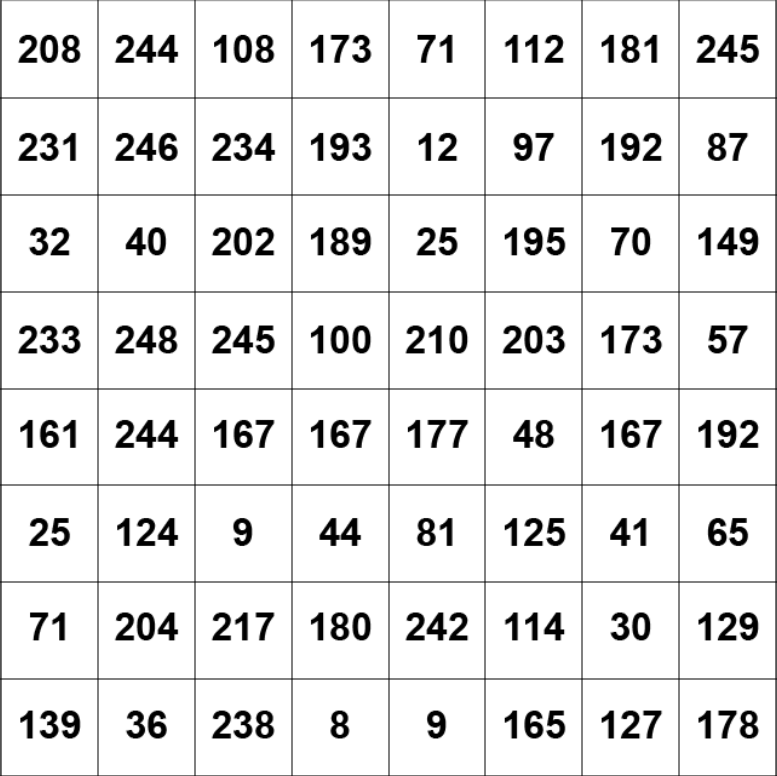
\includegraphics[width=.5\linewidth]{MatrizNivelCinza}
  \caption{}
  \label{exemplo:sfig1}
\end{subfigure}%
\end{figure}


\end{frame}
\begin{frame}
\frametitle{Espaços de cor}
\begin{itemize}
  \item Modelos de representação de cores.
  \item RGB e YCbCr.
  \item Ambos compostos de três canais.
\end{itemize}
\end{frame}

\begin{frame}
\frametitle{RGB}
\begin{itemize}
  \item Canais vermelho(R), verde(G) e azul(B).
  \item Matrizes contém fatores de influência de cada cor na imagem final.
\end{itemize}

	\begin{equation}
			C_{i,j} = p_{i,j,1} . R + p_{i,j,2} . G + p_{i,j,3} . B ,  (1<i<M, 1<j<N)
	\label{eq:corRGB}
	\end{equation}

\end{frame}

\begin{frame}
\frametitle{RGB}

\begin{figure}
  \centering
  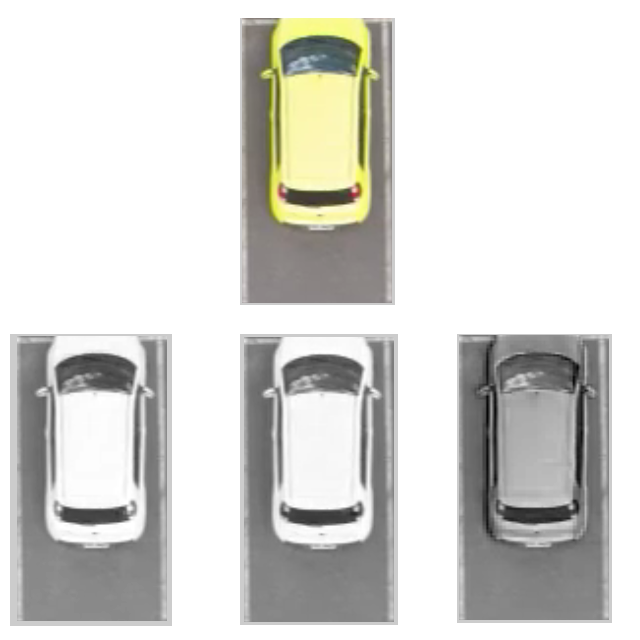
\includegraphics[width=.4\textwidth]{exemploRGBFinal}
  \caption{Uma imagem RGB e seus três canais separados.}
\end{figure}

\end{frame}

\begin{frame}
\frametitle{YCbCr}
\begin{itemize}
\item Usado em vídeos por sua capacidade de compressão.
\item Canais de luminância(Y), crominância azul(Cb) e crominância vermelha(Cr).
\item Pode ser obtida através da imagem RGB.
\item Canais de crominância são gerados pela diferença entre Y e canais R e B. 
\end{itemize}

\begin{equation}
	Y = 0,299.R + 0,587.G + 0,114.B
\label{eq:Y}
\end{equation}

\end{frame}

\begin{frame}
\frametitle{YCbCr}
\begin{figure}
 \centering
 \begin{subfigure}{.2\textwidth}
  \centering
  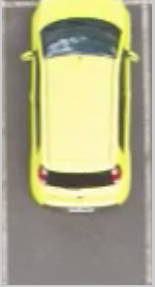
\includegraphics[width=.5\linewidth]{exemploRGB}
\end{subfigure}\
\begin{subfigure}{.2\textwidth}
  \centering
  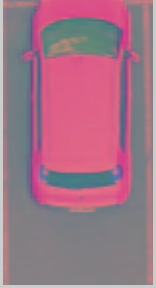
\includegraphics[width=.5\linewidth]{exemploycbcr}
\end{subfigure}
\end{figure}

\begin{figure}
  \centering
  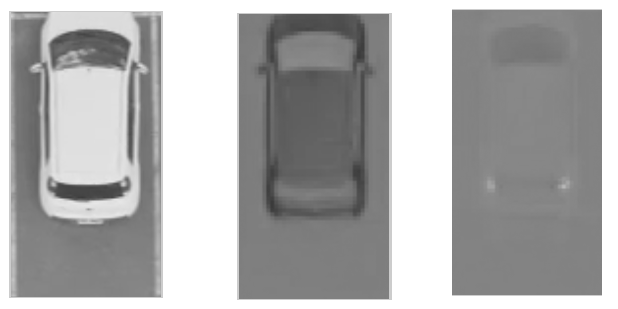
\includegraphics[width=.4\linewidth]{exemploYCbCrFinal}
  \caption{A imagem YCbCr obtida de uma imagem RGB e seus canais.}
\end{figure}
\end{frame}

\begin{frame}
\frametitle{Descritores de textura}
\begin{block}{}
Algoritmos que retorna valores que representam padrões de uma imagem analisada. Analisam a imagem como um todo, ao invés de \textit{pixel-a-pixel}.
\end{block}
\end{frame}

\begin{frame}
\frametitle{GLCM}
\begin{itemize}
\item \textit{Gray Level Co-ocurrence Matrix}.
\item Aplicada em imagens de nível de cinza.
\item Medidas estatísticas.
\item Analisa uma certa relação espacial entre dois \textit{pixels}.
\item Para este trabalho, a relação é a vizinhança direita.
\end{itemize}
\end{frame}

\begin{frame}
\frametitle{GLCM}
\begin{itemize}
\item Saída do algoritmo é uma matriz $MxM$ onde $M$ é o maior nível de cinza possível.
\end{itemize}

\begin{figure}
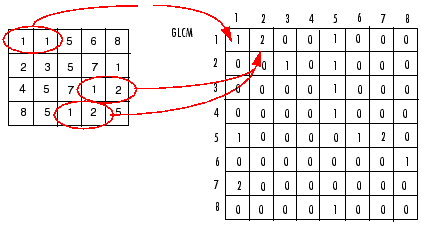
\includegraphics[width=7cm]{GLCM} 
\centering
\caption{Exemplo da elaboração da GLCM. Extraída de https://www.mathworks.com/help/images/ref/graycomatrix.html}
\label{fig:GLCM}
\end{figure}
\end{frame}

\begin{frame}
\frametitle{GLCM}
\begin{block}{Medidas}
\begin{itemize}
\centering
\item[Contraste:] $C = \sum_{i,j} (i-j)^{2}P_{(i,j)}$
\item[Correlação:] $Co = \sum_{i,j} \frac{(i - \mu_i)(j - \mu_j)P_{(i,j)}}{\sigma_i\sigma_j}$
\item[Energia:]$E = \sum_{i,j} P_{(i,j)}^{2}$
\item[Homogeneidade:]$H = \sum_{i,j} \frac{P_{(i,j)}}{1+|i-j|}$
\centering
\end{itemize}
\end{block}
\end{frame}

\begin{frame}
\frametitle{Vídeos}
\begin{block}{Vídeo}
Representação de cenas dinâmicas do mundo real. A sensação de movimento é criada através da exibição de imagens digitais a uma taxa adequada.
\end{block}

\begin{block}{Detecção de Movimento}
Análise da diferença entre dois quadros para estimar a movimentação de objetos na cena.
\end{block}
\end{frame}

\begin{frame}
\frametitle{Fluxo óptico}
\begin{itemize}
\item Estimativa da velocidade do movimento de cada \textit{pixel} da imagem.
\item $I(x,y,t) = I(x+dx, y+dy, t+dt)$
\item Restrição do Fluxo óptico: $\nabla Iv + I_t = 0$.
\item É preciso analisar a vizinhança para encontrar ambos os componentes de $v$.
\item Método Lucas-Kanade: vizinhança local.
\end{itemize}
\end{frame}

\begin{frame}
\frametitle{Fluxo óptico}
\begin{figure}
 \centering
\begin{subfigure}{.4\textwidth}
  \centering
  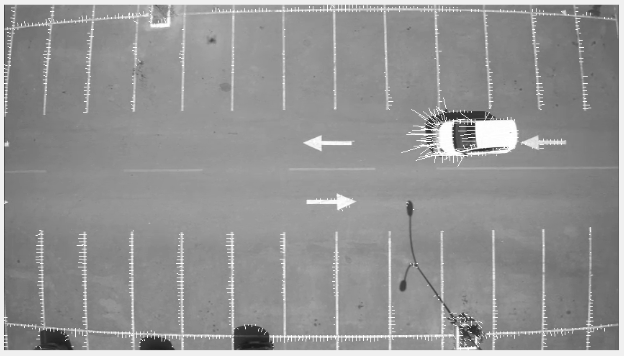
\includegraphics[width=.8\linewidth]{velocidadevetores}
	\caption{}
\end{subfigure}\
\begin{subfigure}{.4\textwidth}
  \centering
  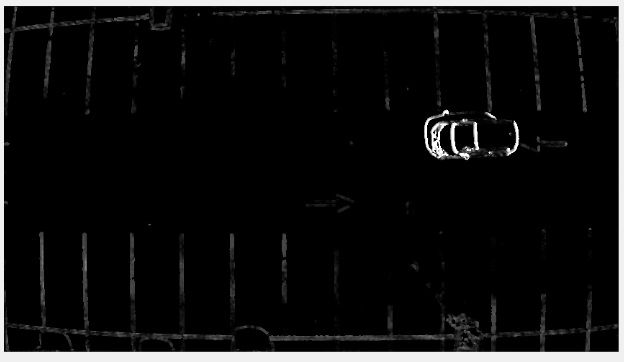
\includegraphics[width=.8\linewidth]{velocidademagnitude}
	\caption{}
\end{subfigure}
\caption{(a) Representação dos vetores de velocidade estimado pelo fluxo óptico. (b) Imagem em níveis de cinza onde a intensidade do \textit{pixel} representa a magnitude do seu vetor de velocidade.}
\end{figure}
\end{frame}

\section{Redes Neurais Artificiais}

\begin{frame}
\frametitle{Redes Neurais Artificias}
\begin{block}{Redes Neurais}
Sistemas inspirados no cérebro humano para realização de tarefas como classificação de padrões e ajuste de funções. Usam elementos de processamento distintos que trabalham paralelamente(neurônios).
\end{block}

\begin{block}{Haykin define como:}
 "...um processador distribuído massivamente paralelo composto por unidades simples de processamento, que possui uma propensidade natural a armazenar conhecimento experimental e torná-lo disponível para uso."
\end{block}
\end{frame}

\begin{frame}
\frametitle{Neurônio}
\begin{figure}
\centering
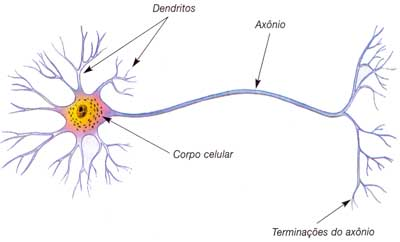
\includegraphics[width=.6\textwidth]{neuronio}
\caption{A estrutura básica de um neurônio humano}
\end{figure}
\end{frame}

\begin{frame}
\frametitle{Neurônio Artificial}
\begin{figure}
\centering
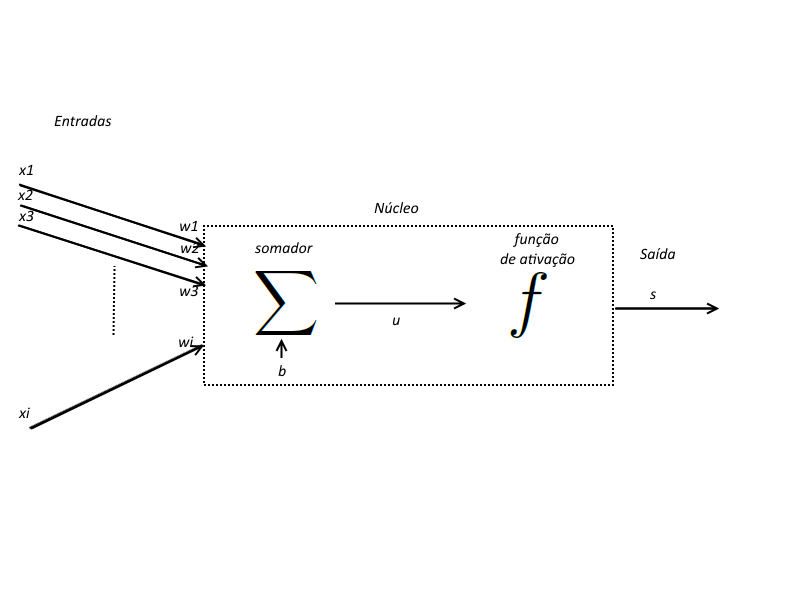
\includegraphics[width=.6\textwidth]{NeuronioArtificial}
\caption{A estrutura básica de um neurônio artificial}
\end{figure}
\end{frame}

\begin{frame}
\frametitle{Arquitetura \textit{Feed-forward}}
\begin{itemize}
\item Arquitetura para organização dos neurônios de uma rede neural artificial.
\item Camada de entrada, camadas ocultas e camada de saída.
\item Informação flui apenas no sentido entrada-saída.
\item Cada neurônio de uma camada é ligado a todos da camada seguinte.
\item Não há ligação entre neurônios de uma mesma camada.
\end{itemize}
\end{frame}

\begin{frame}
\frametitle{Arquitetura \textit{Feed-forward}}
\begin{figure}
\centering
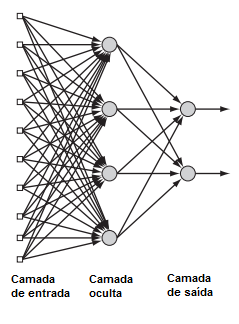
\includegraphics[width=.3\textwidth]{feedforward}
\caption{A arquitetura feed-forward. Adaptada de \cite{Haykin}}
\end{figure}
\end{frame}

\begin{frame}
\frametitle{Treinamento}
\begin{itemize}
\item Processo onde a rede é configurada para realizar a tarefa específica para qual foi criada.
\item Aprendizado: capacidade da rede de aproximar o comportamento das entradas durante o treinamento.
\item Generalização: capacidade da rede de prever e operar sobre entradas que não estavam no conjunto de treinamento.
\item Valores dos pesos $w$ e dos deslocamentos $b$ são definidos.
\end{itemize}
\end{frame}

\begin{frame}
\frametitle{Treinamento}
\begin{itemize}
\item \textbf{Conjunto de treinamento:} Conjunto utilizado para a calibração dos valores de $w$ e $b$.
\item \textbf{Conjunto de validação:} Após cada iteração do treinamento, a rede valida os valores configurados usando este conjunto.
\item \textbf{Conjunto de testes:} A rede é apresentada a este conjunto ao final do treinamento para verificação do funcionamento.
\end{itemize}
\end{frame}

\begin{frame}
\frametitle{Treinamento}
\begin{block}{Treinamento Supervisionado}
Elementos dos conjuntos de treinamento e validação são as entradas e os gabaritos da saídas desejadas de cada entrada. Treina até que a saída seja suficientemente próxima do gabarito.
\end{block}

\begin{block}{Treinamento Não-Supervisionado}
A rede recebe um conjunto de entradas e aprende características intrínsecas dos dados apresentados.
\end{block}

\end{frame}

\begin{frame}
\frametitle{Classificação de padrões}
\begin{itemize}
\item Consiste em analisar padrões de um conjunto de dados e designar o conjunto a uma classe pré-determinada.
\item A rede analisa características ou \textit{features}.
\item \textit{Features} devem ser descritivos e discriminantes.
\item Limiar de decisão.
\item A rede determina a probabilidade de que uma entrada pertença a uma classe.
\end{itemize}
\end{frame}

\begin{frame}
\frametitle{Classificação de padrões}
\begin{figure}
\centering
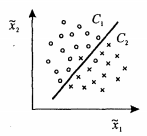
\includegraphics[width=5cm]{features}
\label{fig:features}
\caption{Um gráfico que mostra duas características $\tilde{x}_1$ e $\tilde{x}_2$ de um problema de classificação hipotético. Extraída de \cite{NNForPR}.}
\end{figure}
\end{frame}


\section{Metodologia}

\begin{frame}
\frametitle{Metodologia}
    \begin{block}{Aquisição das imagens}
    Os primeiros testes do trabalho serão feitos sobre imagens criadas artificialmente. Alguns em imagens estáticas e outros em vídeos criados através de manipulação de imagens. Futuramente, vídeos reais serão analisados.
    \end{block}
\end{frame}

\begin{frame}
\frametitle{Metodologia}
    Passos de funcionamento do programa:
    \begin{itemize}
        \item Extração do fundo
        \item Subtração de fundos distintos
        \item Identificação de objetos
    \end{itemize}
\end{frame}

\begin{frame}
\frametitle{Metodologia}
O fundo deve ser gerado de forma dinânica por causa das seguintes dificuldades:
\begin{itemize}
  \item Mudança na iluminação durante o dia
  \item Ruído da imagem
  \item Clima
  \item Objetos novos que podem se integrar ao fundo
\end{itemize}
\end{frame}

\begin{frame}
\frametitle{Metodologia}
    Começa de um fundo inicial.
    Gera o fundo a cada quadro de vídeo segundo a equação:
    \begin{equation}\label{geracaoFundoEquacao}
       Bgi = \left\{
        \begin{array}{l l}
        Ba_{i} & \text{,Fgi=255} \\
        \frac{Bai}{2} + \frac{Qi}{2} & \text{,Fgi=0}\\
         \end{array} \right.
     \end{equation}
\end{frame}

\begin{frame}
\frametitle{Metodologia}
   \begin{figure}
      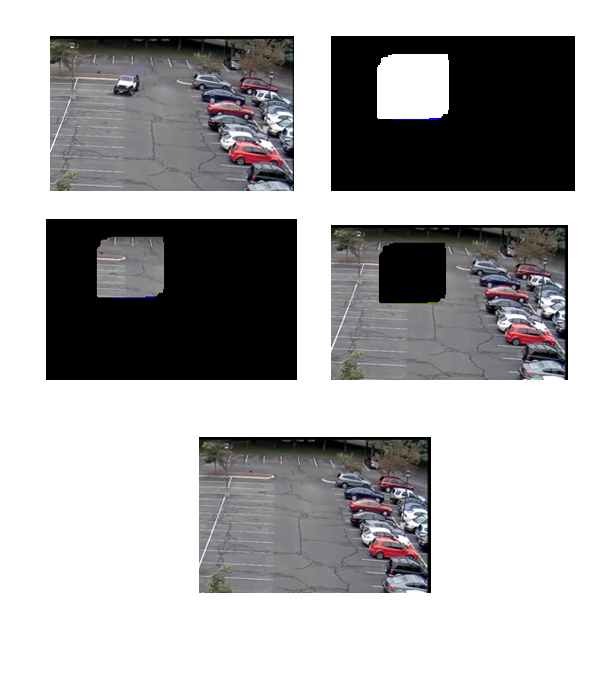
\includegraphics[width=.6\textwidth]{FiguraFundo}
    \end{figure}
\end{frame}

\begin{frame}
\frametitle{Metodologia}
   A cada intervalo de tempo $t$, o fundo atual é subtraído do fundo de $t$ segundos atrás.

   As imagens de diferença são tratadas para excluir diferenças insiginificantes.

   Diferenças podem significar duas coisas:
   \begin{itemize}
        \item Um novo objeto se integrou ao fundo ou;
        \item Um objeto estático saiu da imagem.
    \end{itemize}
\end{frame}

\begin{frame}
\frametitle{Metodologia}
   O próximo passo é comparar a região da diferença com as posições conhecidas de vagas e determinar se a vaga foi ocupada ou desocupada.

   Se o estado anterior é conhecido e apenas carros pudessem se integrar ao fundo, isso seria trivial, mas esse não é o caso.

    Também é preciso identificar que o objeto representado na diferença é realmente um carro.
\end{frame}

\begin{frame}
\frametitle{Metodologia}
   Métodos sendo explorados:
   \begin{itemize}
     \item  Rastreamento
     \item  Comparação de histogramas
     \item  Classificação
   \end{itemize}
\end{frame}

\begin{frame}
\frametitle{Plano de implementação}
   A implementação vai seguir os seguintes passos:
   \begin{itemize}
     \item  Determinar ocupação de vagas em imagens estáticas a partir de um estado inicial conhecido e subtração de imagens.
     \item  Determinar o estado das vagas a partir apenas de uma imagem.
     \item  Usar o segundo passo para conferir os estados obtidos no primeiro passo.
     \item  Implementar os métodos desenvolvidos nos passos anteriores em vídeos 'artificiais'.
     \item  Validar o funcionamento do programa em vídeos reais.
   \end{itemize}
\end{frame}

\section{Cronograma}
\begin{frame}
\frametitle{Cronograma 2015}
%
\begin{tabular}{|l|c|c|c|c|c|c|c|}
\hline
Atividade & Jan & Fev & Mar & Abr & Maio & Jun & Jul \\
\hline
Pesquisa & X & X & & & & &  \\
\hline
Imagens &  & X & X &  &  &  &   \\
\hline
Implementação&  & X & X & X &  &  &   \\
\hline
Validação &   &   &  & X & X &  &   \\
\hline
Análise &   &   &  & X & X & X &   \\
\hline
Escrita  &   &   &  &  & X & X &   \\
\hline
Defesa  &   &   &  &  &  &  & X  \\
\hline
\end{tabular}
%



\end{frame}




\section{Conclusao}
\begin{frame}
\frametitle{Conclusao}
\huge
Perguntas?

\end{frame}


\begin{frame}[allowframebreaks]
\frametitle{Referencias}
\bibliographystyle{plain}
\bibliography{bibliografia}

\end{frame}




\begin{frame}
\frametitle{Conclusao}
\huge
\cite{bong2008integrated} \cite{chen2012dynamic} \cite{de2006introduccao} \cite{delibaltov2013parking}\cite{gonzalez2009digital}
\cite{graciano2007rastreamento} \cite{hai2009self} \cite{IBGE2000introducao} \cite{idris09} \cite{marques1999processamento}
\cite{true2007vacant} \cite{vkl1989jain}
\end{frame}


%------------------------------%


\end{document} 